\documentclass[11pt,a4paper]{article}

\usepackage[left=2.4cm,right=2.4cm,top=2.2cm,bottom=2.2cm]{geometry}

\usepackage[T1]{fontenc}
\usepackage[utf8]{inputenc}
\usepackage{newtxtext,newtxmath}
\usepackage{microtype}

\usepackage{amsmath}
\usepackage{booktabs}
\usepackage{siunitx}
\usepackage{graphicx}
\usepackage{enumitem}

\usepackage[hidelinks]{hyperref}

\sisetup{
  detect-weight = true,
  detect-family = true
}

% Supplementary numbering
\renewcommand{\thetable}{S\arabic{table}}
\renewcommand{\thefigure}{S\arabic{figure}}
\renewcommand{\theequation}{S\arabic{equation}}

\setcounter{secnumdepth}{3}

% Paragraph and line spacing
\setlength{\parindent}{0pt}
\setlength{\parskip}{0.35\baselineskip}
\linespread{1.03}

\begin{document}

\begin{center}
{\Large\bfseries Supplementary Information\par}

\vspace{0.7em}

{\large\bfseries
Physics as the label for measuring and correcting materials reasoning in multimodal models
\par}

\vspace{0.8em}

{\normalsize
Hasan Kurban, Rasul Khanbayov, and Mustafa Kurban
\par}
\end{center}

\vspace{1.0em}

\noindent
This Supplementary Information contains Supplementary Note 1, which provides
the standard derivations underlying the physical oracles and statistical
estimators used in the Article, together with Supplementary Table S1, which
reports the per-cell Physical-Consistency Rate (PCR) and corresponding bootstrap
confidence intervals. Proposition~1 and Corollary~1, which constitute the main
measurement-theoretic result of the study, are stated and proved in the main
Article.

\vspace{0.5em}

\section*{Supplementary Note 1: standard derivations}
\noindent The results collected here are standard and are included for completeness.
\setcounter{subsection}{0}
\renewcommand{\thesubsection}{1.\arabic{subsection}}

\subsection{Bragg's law and \texorpdfstring{$d$}{d}-spacing}
For constructive interference from lattice planes of spacing $d$ at Bragg angle
$\theta$ with a beam of wavelength $\lambda$, the path difference $2d\sin\theta$ equals an
integer number of wavelengths; for first order ($n=1$), $\lambda=2d\sin\theta$. The
measured scattering angle is $2\theta$, so a claimed peak at $2\theta$ corresponds to
$d=\lambda/\!\big(2\sin\theta\big)$ with $\theta$ equal to half the measured angle.
Physical realizability requires $\sin\theta\le1$, equivalently $d\ge\lambda/2$, and the
instrument range further restricts $2\theta$ to a finite window; the diffraction oracle
enforces both and matches claimed peaks to the reference pattern of the stated phase
within tolerance.

\subsection{Scale-bar calibration}
A scale bar of stated length $\ell_{\mathrm{nm}}$ spanning $p_{\mathrm{bar}}$ pixels
fixes the calibration $s=\ell_{\mathrm{nm}}/p_{\mathrm{bar}}$ (nanometres per pixel).
For an image whose long edge is $p_{\mathrm{img}}$ pixels, the field of view is
$s\,p_{\mathrm{img}}$ nanometres, which upper-bounds any reported feature size and
defines the microscopy oracle.

\subsection{Convex-hull stability}
For a given composition, the energy above the convex hull $E_{\mathrm{hull}}\ge0$ is the
formation energy minus that of the lowest-energy combination of stable phases at the
same composition. A phase is thermodynamically stable when $E_{\mathrm{hull}}=0$ and is
treated as within tolerance when $E_{\mathrm{hull}}\le\epsilon$; the DFT-grounded near-hull oracle uses the reported threshold
$\epsilon=0.05\,\mathrm{eV\,atom^{-1}}$.

\subsection{Percentile bootstrap confidence intervals}
For a rate estimated from $n$ items we resample items with replacement $B$ times,
recompute the rate on each resample, and report the empirical $\alpha/2$ and
$1-\alpha/2$ quantiles. Under independent sampling of items the interval is consistent
as $n,B\to\infty$. Where items share a parent source (for example, several questions
about one structure), we resample at the source level to respect that dependence. We
report the interval for all rates.

\subsection{Concentration of the empirical rate}
For a rate $\bar X=\frac1n\sum_{i=1}^n X_i$ that averages independent variables
$X_i\in[0,1]$ with mean $\mathbb{E}[\bar X]=\mu$, Hoeffding's inequality gives
$\Pr[\,|\bar X-\mu|>t\,]\le 2e^{-2nt^2}$ for every $t>0$. Applied to $X_i=1-Y_i$ this
bounds the sampling error of $\mathrm{PCR}^\star$ about the population physical-consistency rate; where items share a parent source, $n$ is the number of independent sources, matching the source-level percentile bootstrap above.

\subsection{Exact McNemar test}
For paired before/after consistency, let $b$ and $c$ be the numbers of discordant items
(consistent-then-inconsistent, i.e.\ regressions, and inconsistent-then-consistent,
i.e.\ fixes). Under the null that each discordant item changes direction with
probability $\tfrac12$, $c\sim\mathrm{Binomial}(b+c,\tfrac12)$, and the two-sided exact
$p$-value is $\min\!\big(1,\,2\sum_{k=0}^{\min(b,c)}\binom{b+c}{k}2^{-(b+c)}\big)$. This
is the test used for CGSV in the main Article.
\subsection{Distribution-free bound on the total error of a reported rate}
The main Article's Proposition~1 and Corollary~1 are exact statements about the oracle's
bias on a fixed set of items. If, in addition, the checkable items are drawn independently
from the benchmark's item-generating process, with
$\mu=\mathbb{E}[1-Y_i]$ that process's physical-consistency rate, then splitting
$\mathrm{PCR}-\mu=(\mathrm{PCR}-\mathrm{PCR}^\star)+(\mathrm{PCR}^\star-\mu)$, bounding the
first term by $(1-\hat d)+\hat f$ (Corollary~1) and the second by the concentration
inequality above gives, for every $t>0$, with probability at least $1-2e^{-2nt^2}$,
\[
|\mathrm{PCR}-\mu|\;\le\;\underbrace{(1-\hat d)+\hat f}_{\text{oracle bias}}\;+\;\underbrace{t}_{\text{sampling}}.
\]
Where items share a parent source the same statement holds with $n$ replaced by the number
$m$ of independent sources under balanced source sizes; unequal sizes give a size-weighted
mean and a correspondingly weaker rate. Both steps are standard, and the independence
assumption is an idealization for a convenience benchmark. At the cell sizes used in the
Article the sampling term is far looser than the percentile bootstrap interval: at $n=90$ and
$95\%$ confidence it is $t=0.143$, against reported per-cell intervals of roughly $\pm0.09$.
The Article therefore reports bootstrap intervals as its uncertainty and uses this bound only
to show that the two sources of error are separately controlled.

\clearpage
\section*{Supplementary Figure S1}
\noindent\textbf{Oracle precision audit, every family, full breakdown.} Referenced from
the main Article's Results (Oracle validity subsection). Each bar is every
human-reviewed oracle-fired case for that family (Article, Table~1), split into real
violations, false positives, and unsure verdicts. Precision is high across the board
(77.2--95.3\%) but not uniform: diffraction's tolerance is visibly the tightest relative
to typical model precision, while the three DFT-grounded families cluster above 92\%.
\begin{figure}[htbp]
\centering
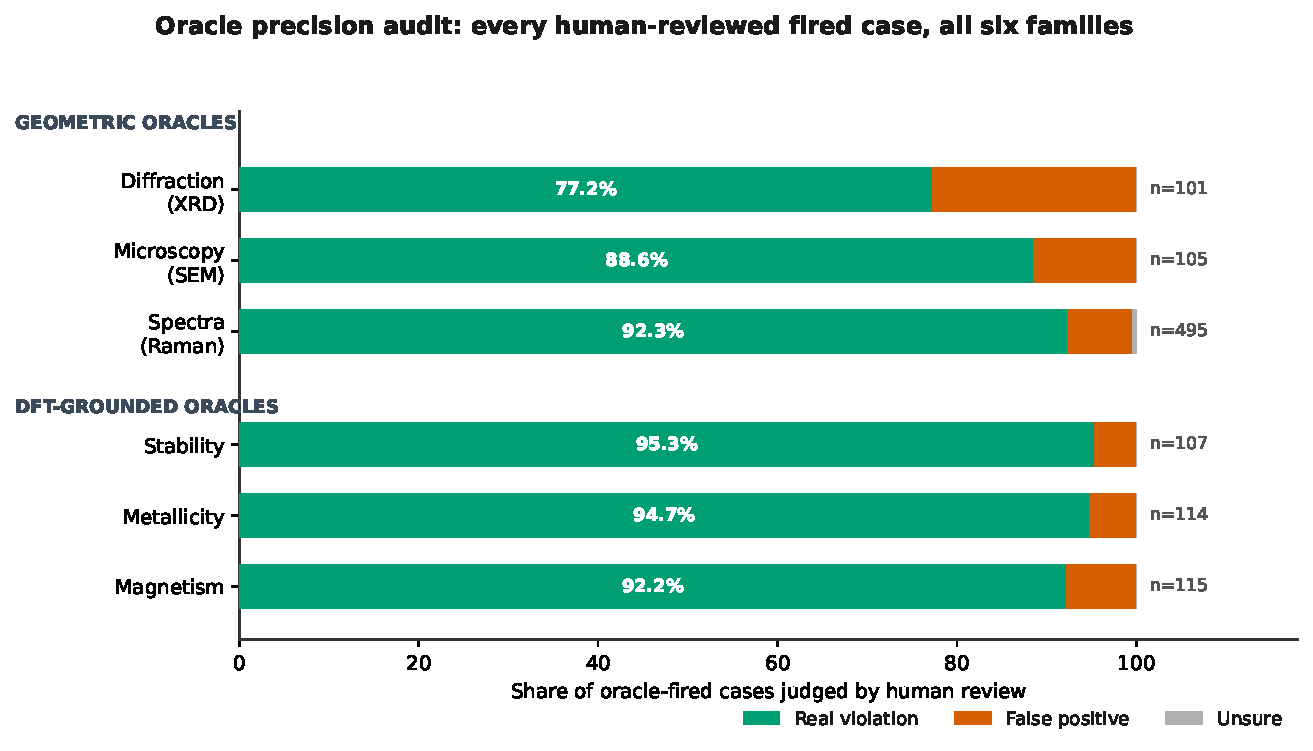
\includegraphics[width=0.92\linewidth]{figures/fig_precision_funnel.pdf}
\label{fig:precision-funnel}
\end{figure}

\clearpage
\section*{Supplementary Table S1}
\noindent\textbf{Per-cell Physical-Consistency Rate with bootstrap 95\% confidence
intervals.} Referenced from the main evaluation table of the Article. $n$ is the number of checkable records in the cell
(pooled across $S=3$ seeds); CI is the percentile bootstrap 95\% interval ($B=10{,}000$
resamples) on the cell's own PCR. The first four models are the originally evaluated set;
the next four are the later-generation refresh; the last (GPT-5.6-Sol) is a flagship-tier
addition testing whether it exceeds the balanced-tier GPT-5.6-Terra within the same
generation (Article, Table~1 note). Each item in this benchmark exposes
exactly one checkable constraint of its own constraint type, so the per-constraint-type
violation rate $\rho_t=1-\mathrm{PCR}$ for every cell below and is not tabulated separately.
\begin{table}[htbp]
\centering
{\scriptsize\setlength{\tabcolsep}{4pt}\renewcommand{\arraystretch}{1.05}
\begin{tabular}{l l S[table-format=3.0] S[table-format=1.3] c}
\toprule
Model & Constraint type & {$n$} & {PCR} & {95\% CI} \\
\midrule
Qwen2.5-VL-7B & Diffraction & 64 & 0.500 & [0.375, 0.625] \\
Qwen2.5-VL-7B & Microscopy & 87 & 0.667 & [0.563, 0.759] \\
Qwen2.5-VL-7B & Spectra & 88 & 0.148 & [0.080, 0.227] \\
Qwen2.5-VL-7B & Stability$^{*}$ & 90 & 0.744 & [0.656, 0.833] \\
Qwen2.5-VL-7B & Metallicity$^{*}$ & 87 & 0.540 & [0.437, 0.644] \\
Qwen2.5-VL-7B & Magnetism$^{*}$ & 90 & 0.767 & [0.678, 0.856] \\
\addlinespace
Gemini 2.5 Flash Lite & Diffraction & 60 & 0.517 & [0.400, 0.650] \\
Gemini 2.5 Flash Lite & Microscopy & 86 & 1.000 & [1.000, 1.000] \\
Gemini 2.5 Flash Lite & Spectra & 90 & 0.278 & [0.189, 0.378] \\
Gemini 2.5 Flash Lite & Stability$^{*}$ & 89 & 0.730 & [0.640, 0.820] \\
Gemini 2.5 Flash Lite & Metallicity$^{*}$ & 84 & 0.702 & [0.607, 0.798] \\
Gemini 2.5 Flash Lite & Magnetism$^{*}$ & 89 & 0.494 & [0.382, 0.596] \\
\addlinespace
GPT-4o & Diffraction & 64 & 0.625 & [0.500, 0.750] \\
GPT-4o & Microscopy & 87 & 0.954 & [0.908, 0.989] \\
GPT-4o & Spectra & 44 & 0.068 & [0.000, 0.159] \\
GPT-4o & Stability$^{*}$ & 90 & 0.800 & [0.711, 0.878] \\
GPT-4o & Metallicity$^{*}$ & 85 & 0.671 & [0.565, 0.765] \\
GPT-4o & Magnetism$^{*}$ & 90 & 0.678 & [0.578, 0.778] \\
\addlinespace
Claude Sonnet 4.5 & Diffraction & 64 & 0.547 & [0.422, 0.672] \\
Claude Sonnet 4.5 & Microscopy & 87 & 0.977 & [0.943, 1.000] \\
Claude Sonnet 4.5 & Spectra & 90 & 0.189 & [0.111, 0.267] \\
Claude Sonnet 4.5 & Stability$^{*}$ & 90 & 0.756 & [0.667, 0.844] \\
Claude Sonnet 4.5 & Metallicity$^{*}$ & 85 & 0.694 & [0.600, 0.788] \\
Claude Sonnet 4.5 & Magnetism$^{*}$ & 90 & 0.756 & [0.666, 0.844] \\
\addlinespace
Claude Opus 4.6 & Diffraction & 64 & 0.578 & [0.453, 0.703] \\
Claude Opus 4.6 & Microscopy & 87 & 0.954 & [0.908, 0.989] \\
Claude Opus 4.6 & Spectra & 90 & 0.244 & [0.156, 0.333] \\
Claude Opus 4.6 & Stability$^{*}$ & 90 & 0.722 & [0.633, 0.811] \\
Claude Opus 4.6 & Metallicity$^{*}$ & 86 & 0.721 & [0.628, 0.814] \\
Claude Opus 4.6 & Magnetism$^{*}$ & 90 & 0.700 & [0.600, 0.789] \\
\addlinespace
GPT-5.6-Terra & Diffraction & 64 & 0.797 & [0.703, 0.891] \\
GPT-5.6-Terra & Microscopy & 81 & 0.951 & [0.901, 0.988] \\
GPT-5.6-Terra & Spectra & 90 & 0.833 & [0.756, 0.911] \\
GPT-5.6-Terra & Stability$^{*}$ & 90 & 0.656 & [0.556, 0.756] \\
GPT-5.6-Terra & Metallicity$^{*}$ & 85 & 0.659 & [0.553, 0.753] \\
GPT-5.6-Terra & Magnetism$^{*}$ & 90 & 0.767 & [0.678, 0.844] \\
\addlinespace
Qwen3-VL-8B-Instruct & Diffraction & 62 & 0.468 & [0.355, 0.597] \\
Qwen3-VL-8B-Instruct & Microscopy & 86 & 0.802 & [0.709, 0.884] \\
Qwen3-VL-8B-Instruct & Spectra & 90 & 0.133 & [0.067, 0.200] \\
Qwen3-VL-8B-Instruct & Stability$^{*}$ & 87 & 0.713 & [0.621, 0.805] \\
Qwen3-VL-8B-Instruct & Metallicity$^{*}$ & 77 & 0.688 & [0.584, 0.792] \\
Qwen3-VL-8B-Instruct & Magnetism$^{*}$ & 90 & 0.533 & [0.433, 0.633] \\
\addlinespace
Qwen3-VL-8B-Thinking & Diffraction & 64 & 0.578 & [0.453, 0.703] \\
Qwen3-VL-8B-Thinking & Microscopy & 87 & 0.885 & [0.816, 0.943] \\
Qwen3-VL-8B-Thinking & Spectra & 87 & 0.092 & [0.034, 0.161] \\
Qwen3-VL-8B-Thinking & Stability$^{*}$ & 90 & 0.767 & [0.678, 0.856] \\
Qwen3-VL-8B-Thinking & Metallicity$^{*}$ & 87 & 0.644 & [0.540, 0.736] \\
Qwen3-VL-8B-Thinking & Magnetism$^{*}$ & 89 & 0.506 & [0.404, 0.607] \\
\addlinespace
GPT-5.6-Sol & Diffraction & 61 & 0.820 & [0.721, 0.918] \\
GPT-5.6-Sol & Microscopy & 82 & 0.915 & [0.854, 0.976] \\
GPT-5.6-Sol & Spectra & 89 & 0.764 & [0.674, 0.854] \\
GPT-5.6-Sol & Stability$^{*}$ & 89 & 0.742 & [0.652, 0.831] \\
GPT-5.6-Sol & Metallicity$^{*}$ & 88 & 0.670 & [0.580, 0.761] \\
GPT-5.6-Sol & Magnetism$^{*}$ & 90 & 0.733 & [0.644, 0.822] \\
\bottomrule
\end{tabular}}
\end{table}
\end{document}
